\documentclass{article}
\usepackage[nonumberlist]{glossaries}
\usepackage{graphicx}

\newglossaryentry{generation}
{
    name = Procedural Generation,
    description = {The generation of game elements during runtime}
}

\newglossaryentry{runtime}
{
    name = Runtime,
    description = {The time in which the game code is running}
}

\newglossaryentry{rogue}
{
    name = RogueLike,
    description = {The time in which the game code is running}
}

\newglossaryentry{tilemap}
{
    name = {tilemap},
    description = {The sprites used to make the map of the game.}
}

\newglossaryentry{objective}
{
    name = {Objective},
    description = {The area which the player needs to bring the key.}
}

\newglossaryentry{element}
{
    name = {game element},
    description = {A part of the game.}
}

\newglossaryentry{RandomWalk}
{
    name = {Random Walk Agent},
    description = {Way to keep track of where the algorithm is currently at}
}

\begin{document}

\section*{Hypothesis}
Will the introduction of a rogue-like level generation complement the horror themes of the game
or will it remove the player from the immersion of the game.

\section*{Goal}
The goal of this prototype is to make a procedural generation algorithm that generates a 
level for the player. 
The algorithm needs to make different rooms that connect to each other while also generating
lights in each rooms. The algorithm will also need to generate a key room which holds a key that
the player needs to pick up, along with a door room which the player needs to bring the key towards.
The algorithm will be considered a success if 
\begin{itemize}
    \item All rooms can be accessed.
    \item The player cannot escape the level.
    \item The key is created correctly.
    \item The door is created correctly.
    \item There are lights in the room.
    \item The enemy AI made in prototype 3 can navigate the level.
    \item The correct generation is consistent.
\end{itemize}

\section*{Challenges}
The general objective of the prototype is to find a key that opens a door in a dungeon like structure, 
while avoiding an enemy AI that is trying to hunt the player.
Some challenges the player may face while trying to complete their objectives
\begin{itemize}
    \item Finding out where the key is.
    \item Evading the enemy.
    \item Hiding from the enemy.
    \item Finding the door that the key unlocks.
\end{itemize}

\section*{Mechanics}
The mechanics that the player can use were shown in previous documents.
Here is a summary of the mechanics that the player can use:
\begin{itemize}
    \item Move with WASD.
    \item Sprint with LShift.
    \item Interact with various game elements through Space.
    \item Toggle the player light with R.
\end{itemize}
\section*{Balance}
The movement mechanic has been balanced in such a way that the base player movement speed is slower
than the base enemy movement speed this is to force the player to use their sprint to get always
or to avoid the enemy entirely. 
The sprint mechanic can only be used for a second just to quickly get away form the enemy this
shows the player that it is better to avoid the enemy than to run from them.
The player can only interact with one interaction at a time this forces the player to drop the item 
they are carrying before interacting with another interaction.


\section*{Games with procedural generation}
\subsection*{The Binding of Isaac}
The Binding of Isaac uses a 9x8 grid with each grid cell numbered. The top left grid cell is 0 while
the bottom right cell is 79, this is kept track of with a one dimensional array of 80 length where
the units digit is the x position and the tens digit is the y position on the grid. The algorithm 
for The Binding of Isaac then chooses a random number of rooms to fit in this grid. It always places
the starting room at grid space 35. It then determines the neighbor of the starting room by adding
+1/-1/+10/-10 , if the algorithm can't place a room it gives up. The algorithm keeps track of dead end
rooms which is a room that does not add any neighbors. The algorithm then decides to put special rooms
on the dead end rooms. There are always one of any special room in a level.

I want to take the dead end rooms that only have one entrance and exit and then put then to be either the 
key room or the door room.

\section*{Genre}
The genre of the game is horror, because the player will need to run from an enemy that is hunting them.
The gameplay is inspired by Alien: Isolation which is discussed in more detail from the previous prototype
game design document. 
This prototype explores the RogueLike genre more by using procedural generation to make each playthrough 
different. The core gameplay of hiding from the enemy while trying to move a key to an objective stays the
same only the map changes every time.

\section*{Different Procedural Generation Algorithms}
These algorithms will help in creating the procedural generation algorithm for the prototype.
\subsection*{Binary Space Partitioning}
Binary Space Partitioning is a technique to generate procedural dungeons. It does this by
recursively dividing a large area into smaller non overlapping areas. 
The algorithm does this by making a single rectangular map then it chooses a random direction
and position along the axis and then splits the rectangular map. It repeats this procedure
until the number of rectangular that you want are met. It also makes sure that it does not
split the rectangles beyond a minimum, thus the rectangles will always have a minimum size.
When the entire rectangle has been split the algorithm then shrinks each rectangle to finish
the level generation.
Pros:
\begin{itemize}
    \item No rooms will overlap.
    \item Rooms are guaranteed to be able to reach each other.
\end{itemize}
Cons:
\begin{itemize}
    \item Can only generate rectangular rooms.
    \item Can not generate hallways between rooms.
\end{itemize}

\subsection*{Wave Function Collapse}
Wave Function Collapse (WFC) is an algorithm based on constraints. The function ensures consistency
through adjacency rules which determine which tiles can be placed next to each other. The 
function takes a sample input and generates similar to the sample inputs. The functions
picks a cell at random and then collapses it by choosing a random tile. It then chooses
a grid space next to the chosen tile with the least entropy, least amount of tile options.
This process of collapsing repeats until the entire grid is collapsed or a contradiction 
appears when the algorithm cannot find any possible tiles to place down, leading the program
to either backtrack or start from the beginning.
Pros:
\begin{itemize}
    \item Makes natural looking maps.
\end{itemize}
Cons
\begin{itemize}
    \item Takes a lot of processing power
    \item May be prone to contradictions.
\end{itemize}

\subsection*{Random Walk}
Random Walk is when an agent randomly walks around. The algorithm takes in a walklength and how many times
it should walk this walklength. It is one of the most simple procedural generation algorithms.
Pros:
\begin{itemize}
    \item Makes organic looking caves.
    \item Very easy to setup.
\end{itemize}
Cons:
\begin{itemize}
    \item Can leave some spots open causing a disconnect in the floor
    \item Generation can fail due to randomness.
\end{itemize}

\section*{Procedural Generation Algorithm}
The algorithm I will make will follow the Binary Space Partitioning first to get the rooms
and their layout. 
Then it will connect the rooms together with hallways. It will do this by choosing a room in the middle 
and branching out. If the distance between two rooms are too big it will not connect the hallway between
them.
The algorithm will keep track of rooms with only one entrance to them and then choose those rooms to
be key or door rooms. If there are not enough single entrance rooms then the algorithm will check which
room has two hallways and then will remove one hallway. If there are not enough two hallway rooms
it will remove from three hallway rooms.
After it has mapped out the rooms and hallways it will then place the tiles for the floor from the tilemap.
After it has placed the floor it will place the walls around the floors.
The algorithm will then place the lights scarcely throughout the map on the floor.
It will also place hiding spots scarcely throughout the map on the walls.
It will then place the player randomly and then will place the enemy as far away from the player as possible.


\section*{Macro Design}
The overall goal that the player needs to achieve is to escape. To achieve this goal the player will need
to explore the map to find a key to be able to open the exit. An enemy will chase the player while they are
searching for the key and exit.
The overall story of the game is that the player found themselves in some sort of laboratory and they need to escape.
The player can escape quickly if they follow the voice of the narrator from prototype 1, but if they defy the narrator
it leads the player to the level in prototype 3. The player would then need to escape from their own consequences.
The level of the prototype is made through a procedural generation algorithm using BSP. This will cause the rooms in 
the levels to take on a rectangular shape.


\section*{Process}
WFC was not used during the process of making the room generation algorithm. This is because the game has no
decorations for the level which limits the effectiveness of WFC, because it works best when making predetermined 
tile patterns. The entire level is procedurally generated so there are no predetermined tile patterns.

The algorithm corridor generation differed from the original plan of selecting a singular room and then branching out
from that room. The algorithm has a list of all the rooms and then chooses the first room in the list then it finds the 
closest room that is a part of the room list. It then removes that room from the room list and connects the current room
the the closest room. It continues doing this until the room list is empty.
I made this change because it ensures that the rooms are all connected in a more realistic way by allowing all the rooms
to have the same amount of emphasis instead of putting the most emphasis on the centre room. This shows the player that
all the rooms are important and not just one room is important.

The algorithm for the BSP chooses a dungeon rectangle and then splits it until it can't split the rectangle anymore.
Each split is a room and the algorithm will never split the rooms below a specified size. The sizes chosen for the map
is 200 units by 200 units, while the minimum room size is set to 15 units by 15 units. The 200 x 200 size was chosen
because it allows enough 15 x 15 rooms so that the player still has to traverse the map to get to the objective. Another
reason is that the enemy needs to move through different rooms to make the player feel like they are being hunted.
The 15 x 15 minimum room choice is to make the rooms not feel claustrophobic, but still small enough to make traversing
the map a chore.
After playtesting it was found that a 150 by 150 map was more reasonable for players to navigate while a minimum room of
20 by 20 allows easer escaping from the enemy.

The algorithm uses random walk with two important variables: iterations and walk length. Iterations is how many times the 
algorithm should randomly walk while walk length is how far the algorithm walks per iteration. The higher the iteration the
more likely the end generation to be a square of walk length. The numbers chosen for iterations is 100 while the walk length
is 50. These values where chosen, because if a room is the minimum size of 15x15 it will be a rectangle, but the bigger rooms
will look as if they are decaying which gives the player a feeling of eeriness.

\begin{figure}[ht!]
    \centering
    \begin{minipage}[b]{0.4\textwidth}
        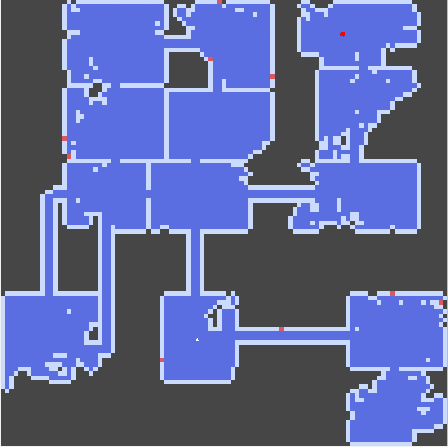
\includegraphics[width=\textwidth]{Images/RandomWalkGeneration.png}
        \caption{Random Walk Generation}
        \label{img:RandomWalk}
    \end{minipage}
    \hfill
    \begin{minipage}[b]{0.4\textwidth}
            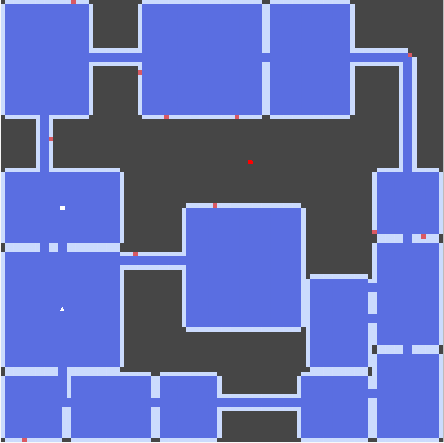
\includegraphics[width=\textwidth]{Images/BinarySpacePartitioning.png}
            \caption{No Random Walk Generation}
            \label{img:BinarySpacePartitioning}
    \end{minipage}
\end{figure}

The algorithm does not keep track of rooms with only 1 entrance/exit to place the key and objective, rather the algorithm randomly
places the key and then places the objective as far away from the key as possible. 

Another devtool was added in order to help show off the map generation. This is to more easily find if the generation achieved
the generation goals listed in Goals.


\section*{Reflection}
The making of the algorithm was easy the hard part was tuning the values to get a result that works for the game. If the values
were too low for the random walk algorithm the rooms will be generated too small and with random walls stopping the flow of movement
with walls placed in the middle of the rooms. With larger values the walls that are randomly placed within the room act as hiding
spots for the player.

One problem with the procedural generation is that some generations cause the player to have to move around the enemy in order to
progress. This is a bit frustrating because you either have to wait in a hiding spot or try to manoeuver around the enemy which can
increase the games difficulty. To fix this problem the algorithm would then need to keep track of the amount of entrances to the rooms.
This can be an improvement of the project in the future.

The RogueLike elements does add to the eeriness of the level, but it can be just as annoying and frustrating when the algorithm 
generates in a way that disadvantages the player causing them to lose the game quickly. Some ways to improve on this is to use 
the Wave Function Collapse algorithm because if the function is given a input of the wanted end result then the algorithm can
clean up the generated rooms and stop unwanted generations.

All the algorithms researched have their own strengths and weaknesses. If the algorithms are used to their strengths to make
up for the other algorithms' weaknesses then the procedural generation can improve.

\section*{References}
[1]Boris, “Dungeon Generation in Binding of Isaac,” BorisTheBrave.com, Sep. 12, 2020. https://www.boristhebrave.com/2020/09/12/dungeon-generation-in-binding-of-isaac/
[2]“Procedural Generation with Wave Function Collapse and Model Synthesis | Unity Devlog,” www.youtube.com. https://www.youtube.com/watch?v=zIRTOgfsjl0 (accessed Jun. 08, 2023).
‌[3]Sunny Valley Studio, “Binary Space Partitioning Algorithm - P13 - Unity Procedural Generation of a 2D Dungeon,” YouTube, Dec. 19, 2020. https://www.youtube.com/watch?v=nbi88hY9hcw (accessed Apr. 28, 2026).
[4]“Generating a 2D map using the Random Walk algorithm | Noveltech,” sveltekit-prerender, Jul. 17, 2023. https://www.noveltech.dev/procgen-random-walk
‌
\glsaddall
\printglossary

\end{document}